% !TEX root = _main.tex

\begin{figure*}[tb]
	\centering
	\begin{minipage}{0.36\hsize}
		\centering
		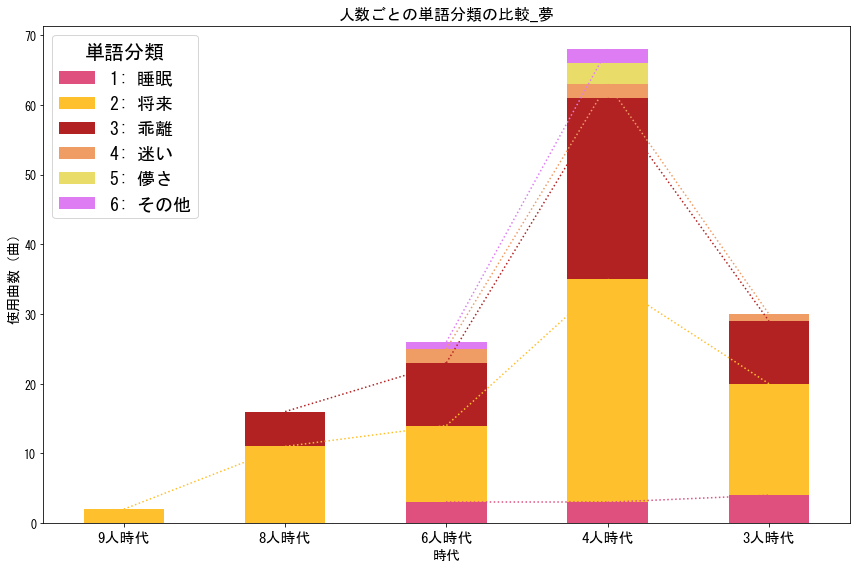
\includegraphics[width=\hsize]{fig/yume-ninzu.png}
		\caption{「夢」人数時代別使用意味比較}
		\label{fig:yume-ninzu}
	\end{minipage}
	\begin{minipage}{0.62\hsize}
		\centering
		\scriptsize
		\captionof{table}{「夢」人数別時代ごとの\kyokusu （()内は割合）}
		\label{tab:yume-uchi}
		\begin{tabular}{c|cccccc}
			\hline
			「夢」の分類 & ９人時代      & ８人時代      & ６人時代      & ４人時代      & ３人時代      & 合計        \\
			\hline\hline
			1:睡眠   & 0 (0.0)   & 0 (0.0)   & 3 (11.5)  & 3 (4.4)   & 4 (13.3)  & 10 (7.0)  \\
			2:将来   & 2 (100.0) & 11 (68.8) & 11 (42.3) & 32 (47.1) & 16 (53.3) & 72 (50.7) \\
			3:乖離   & 0 (0.0)   & 5 (31.2)  & 9 (34.6)  & 26 (38.2) & 9 (30.0)  & 49 (34.5) \\
			4:迷い   & 0 (0.0)   & 0 (0.0)   & 2 (7.7)   & 2 (2.9)   & 1  (3.3)  & 5 (3.5)   \\
			5:儚さ   & 0 (0.0)   & 0 (0.0)   & 0 (0.0)   & 3 (4.4)   & 0 (0.0)   & 3 (2.1)   \\
			6:その他  & 0 (0.0)   & 0 (0.0)   & 1 (3.8)   & 2 (2.9)   & 0 (0.0)   & 3 (2.1)   \\
			\hline
			合計     & 2         & 16        & 26        & 68        & 30        & 142       \\
			\hline
		\end{tabular}
	\end{minipage}
\end{figure*}
